\documentclass[11pt]{article}
\usepackage{cite}
\usepackage{textcomp}
\usepackage{xcolor}
\usepackage{amssymb,times,enumerate,amsmath,subfigure,graphicx,color,ifthen,amsfonts,url}
\usepackage{algorithm,algorithmic,stmaryrd,newfile,mathtools,bm}
%\usepackage{mathtools,amsthm,amssymb}
\usepackage{paralist}


\renewcommand{\sfdefault}{QTCaslanOpen} % TeX Gyre Adventor has small caps
%\newtheorem{theorem}{Theorem}[section]
%\newtheorem{corollary}{Corollary}[theorem]
%\newtheorem{lemma}[theorem]{Lemma}

\usepackage[english]{babel}
\usepackage[utf8]{inputenc}

\usepackage{listings}
\definecolor{mygreen}{rgb}{0,0.2,0}
\definecolor{mygray}{rgb}{0.5,0.5,0.5}
\definecolor{mymauve}{rgb}{0.58,0,0.82}
\definecolor{mypurple}{rgb}{0.38,0,0.32}
\definecolor{myblue}{rgb}{0.1,0,0.32}
\newcommand{\costyle}{\footnotesize\ttfamily\bfseries}
\newcommand{\kwstyle}{\costyle\textcolor{myblue}}
\newcommand{\const}{}
\newcommand{\lt}{\left}
\newcommand{\rt}{\right}
\newcommand{\defeq}{\coloneqq}
\newcommand{\B}[1]{\bm{#1}}
\newcommand{\CC}[1]{\bm{\mathcal{#1}}}
\newcommand{\CD}{\small\ttfamily\bfseries}
\newcommand{\vcr}[1]{\bm{#1}}
\newcommand{\mat}[1]{\bm{#1}}
\newcommand{\tsr}[1]{\bm{\mathcal{#1}}}
\newcommand{\grp}[1]{\bm{\mathcal{#1}}}
\newcommand{\dlt}[1]{\tsr{\partial}^{(#1)}}
\newcommand{\coeff}[1]{\vcr{c}^{(#1)}}
\newcommand{\ecoeff}[1]{c^{(#1)}}
\newcommand{\edlt}[1]{\partial^{(#1)}}
%\newcommand{\rem}[1]{R^{(#1)}}
\newcommand{\rem}[1]{0}

\lstset{ %
  postbreak=false,
%  backgroundcolor=\color{white},   % choose the background color; you must add \usepackage{color} or \usepackage{xcolor}
  basicstyle=\costyle,        % the size of the fonts that are used for the code
%  breakatwhitespace=false,         % sets if automatic breaks should only happen at whitespace
%  breaklines=false,                 % sets automatic line breaking
  captionpos=n,                    % sets the caption-position to bottom
  commentstyle=\color{mygreen},    % comment style
  deletekeywords={...},            % if you want to delete keywords from the given language
  escapeinside={\%*}{*)},          % if you want to add LaTeX within your code
  extendedchars=true,              % lets you use non-ASCII characters; for 8-bits encodings only, does not work with UTF-8
  frame=tb,                    % adds a frame around the code
  keepspaces=true,                 % keeps spaces in text, useful for keeping indentation of code (possibly needs columns=flexible)
  keywordstyle=\color{mypurple},       % keyword style
  language=C++,                 % the language of the code
  otherkeywords={*,...},            % if you want to add more keywords to the set
  numbers=none,                    % where to put the line-numbers; possible values are (none, left, right)
  numbersep=5pt,                   % how far the line-numbers are from the code
  numberstyle=\tiny\color{mygray}, % the style that is used for the line-numbers
  rulecolor=\color{black},         % if not set, the frame-color may be changed on line-breaks within not-black text (e.g. comments (green here))
  showspaces=false,                % show spaces everywhere adding particular underscores; it overrides 'showstringspaces'
  showstringspaces=false,          % underline spaces within strings only
  showtabs=false,                  % show tabs within strings adding particular underscores
  stepnumber=2,                    % the step between two line-numbers. If it's 1, each line will be numbered
  stringstyle=\color{mymauve},     % string literal style
  tabsize=2,                     % sets default tabsize to 2 spaces
  title=\lstname,                   % show the filename of files included with \lstinputlisting; also try caption instead of title
  emph={Set,Monoid,Group,Semiring,Ring,Scalar,Vector,Matrix,Tensor,World,Idx_Tensor,Endomorphism,Univariate_Function,Function,Transform,write,norm2,ctf,tensor,numpy,np,float64,sp,True,reshape,dtype,T,einsum,transpose,tensordot,ndarray,linalg,TTTP,None,sample,i,copy},
  emphstyle=\kwstyle
}



\definecolor{dkgreen}{rgb}{0,0.6,0}
\definecolor{gray}{rgb}{0.5,0.5,0.5}
\definecolor{mauve}{rgb}{0.58,0,0.82}

\lstset{frame=tb,
  language=Java,
  aboveskip=3mm,
  belowskip=3mm,
  showstringspaces=false,
  columns=flexible,
  basicstyle={\small\ttfamily},
  numbers=none,
  numberstyle=\tiny\color{gray},
  keywordstyle=\color{blue},
  commentstyle=\color{dkgreen},
  stringstyle=\color{mauve},
  breaklines=true,
  breakatwhitespace=true,
  tabsize=3
}

\usepackage{geometry}
\geometry{letterpaper}
\usepackage{hyperref}
\hypersetup{
    colorlinks=true,
    linkcolor=blue,
    filecolor=magenta,      
    urlcolor=cyan,
}
\urlstyle{same}

\author{}

\title{}

\begin{document}

\title{Coarsening Schemes}
\maketitle

We are given an undirected, weighted graph $G = (V, E, w)$ where $w: E \to \mathbb{R}$ assigns weights to each edge.\\

As background, we define $\partial(S)$ as the set of edges with exactly one vertex in $S$ and $d(S)$ as the sum of the weighted degrees of vertices in $S$ for any subset $S \subset V$.\\

We begin by defining two key graph metrics.$^1$
\begin{enumerate}
        \item{\bf{Conductance:}} $\phi_G := \min\limits_{S \subset V} \frac{w(\partial (s)))}{\min{(d(S), d(V - S))}}$
        \item{\bf{Stretch:}} $st_T(e) := w_e \sum\limits_{f \in P} \frac{1}{w_f}$ where $P$ is the set of edges in the path from $u$ to $v$ in the spanning tree $T$.
\end{enumerate}

Cheeger's inequality $2 \phi_G \geq \lambda_2 (D^{-1/2}LD^{-1/2}) \geq \frac{\phi_G^2}{2}$ (where $\lambda_2$ is the smallest non-zero eigenvalue) suggests seeking to design Laplacian precondioners with high conductance.\\

We will also see low-stretch subgraphs are good preconditioners.\\

We now identify 3 possible coarsening schemes:
\begin{enumerate}
        \item{\bf{Ultra-sparsifiers}}
        \item{\bf{Bourgain's embedding into $l_1$}}
        \item{\bf{Low-stretch subgraphs}}
\end{enumerate}

\section{Ultra-sparsifiers}
Vaidya studied spanning trees as preconditioners and derived an $O(\sqrt{nm})$ upper bound on the number of iterations of PCG. As we know PCG converges in at most $n$ iterations, spanning trees do not lead to provably fast preconditioners.\\
\newline
Instead, Vaidya suggested "starting" with a spanning tree and adding $O(n)$ edges back to it, with the goal to "fix" eigenvalues. We obtain a tree-like graph and may next do Cholesky factorization to eliminate nodes of degree 1 or 2 and recurse to the next coarser level.$^1$

\section{Bourgain's embedding into $l_1$} To solve min-cost flow, Sherman first embeds the graph into an $l_1$ lattice. Next, they satisfy demands on the near the edges and recurse on the middle.$^2$

\section{Low-stretch subgraphs} Low-strech subgraphs are also known to be good preconditioners. In particular, Sherman uses $j-trees$ (the union of a forest together with another graph) to satisfy max flow demands on the "tree" vertices and recurses on the remaining "interior" graph with more complex structure. Note that low-stretch subgraphs rely heavily on a low-diameter decomposition. $^5$

\section{References}
\begin{enumerate}
        \item{} \href{http://www.cs.yale.edu/homes/spielman/PAPERS/icm10post.pdf}{Algorithms, Graph Theory, and Linear Equations in Laplacian Matrices (Spielman)} provides an overview of the background, ultra-sparsifiers (Section 7), and low stretch spanning trees (Section 6).

        \item{} \href{https://epubs.siam.org/doi/pdf/10.1137/1.9781611974782.49}{Generalized Preconditioning and Undirected Minimum-Cost Flow (Sherman)} provides a framework for the composition of solvers (Section 3) and Bourgain's embedding into $l_1$.

        \item{} \href{https://www.cs.cmu.edu/~guyb/papers/BGKMPT14.pdf}{Nearly-Linear Work Parallel SDD Solvers, Low-Diameter Decomposition, and Low-Stretch Subgraphs (Spielman)}

        \item{} \href{https://people.csail.mit.edu/madry/docs/thesis.pdf}{From Graphs to Matrices, and Back: New Techniques for Graph Algorithms (Madry)}

        \item{} \href{https://arxiv.org/pdf/1304.2077.pdf}{Nearly Maximum Flows in Nearly Linear Time (Sherman)}

        \item{} \href{https://arxiv.org/abs/1911.01956}{Parallel Approximate Undirected Shortest Paths via Low Hop Emulators (Andoni)} provides fast parallel algorithms for Bourgain's embedding (Appendix E) and low diameter decomposition (Appendix F).
\end{enumerate}

\section{Drawings}
\begin{figure}
  \centering
  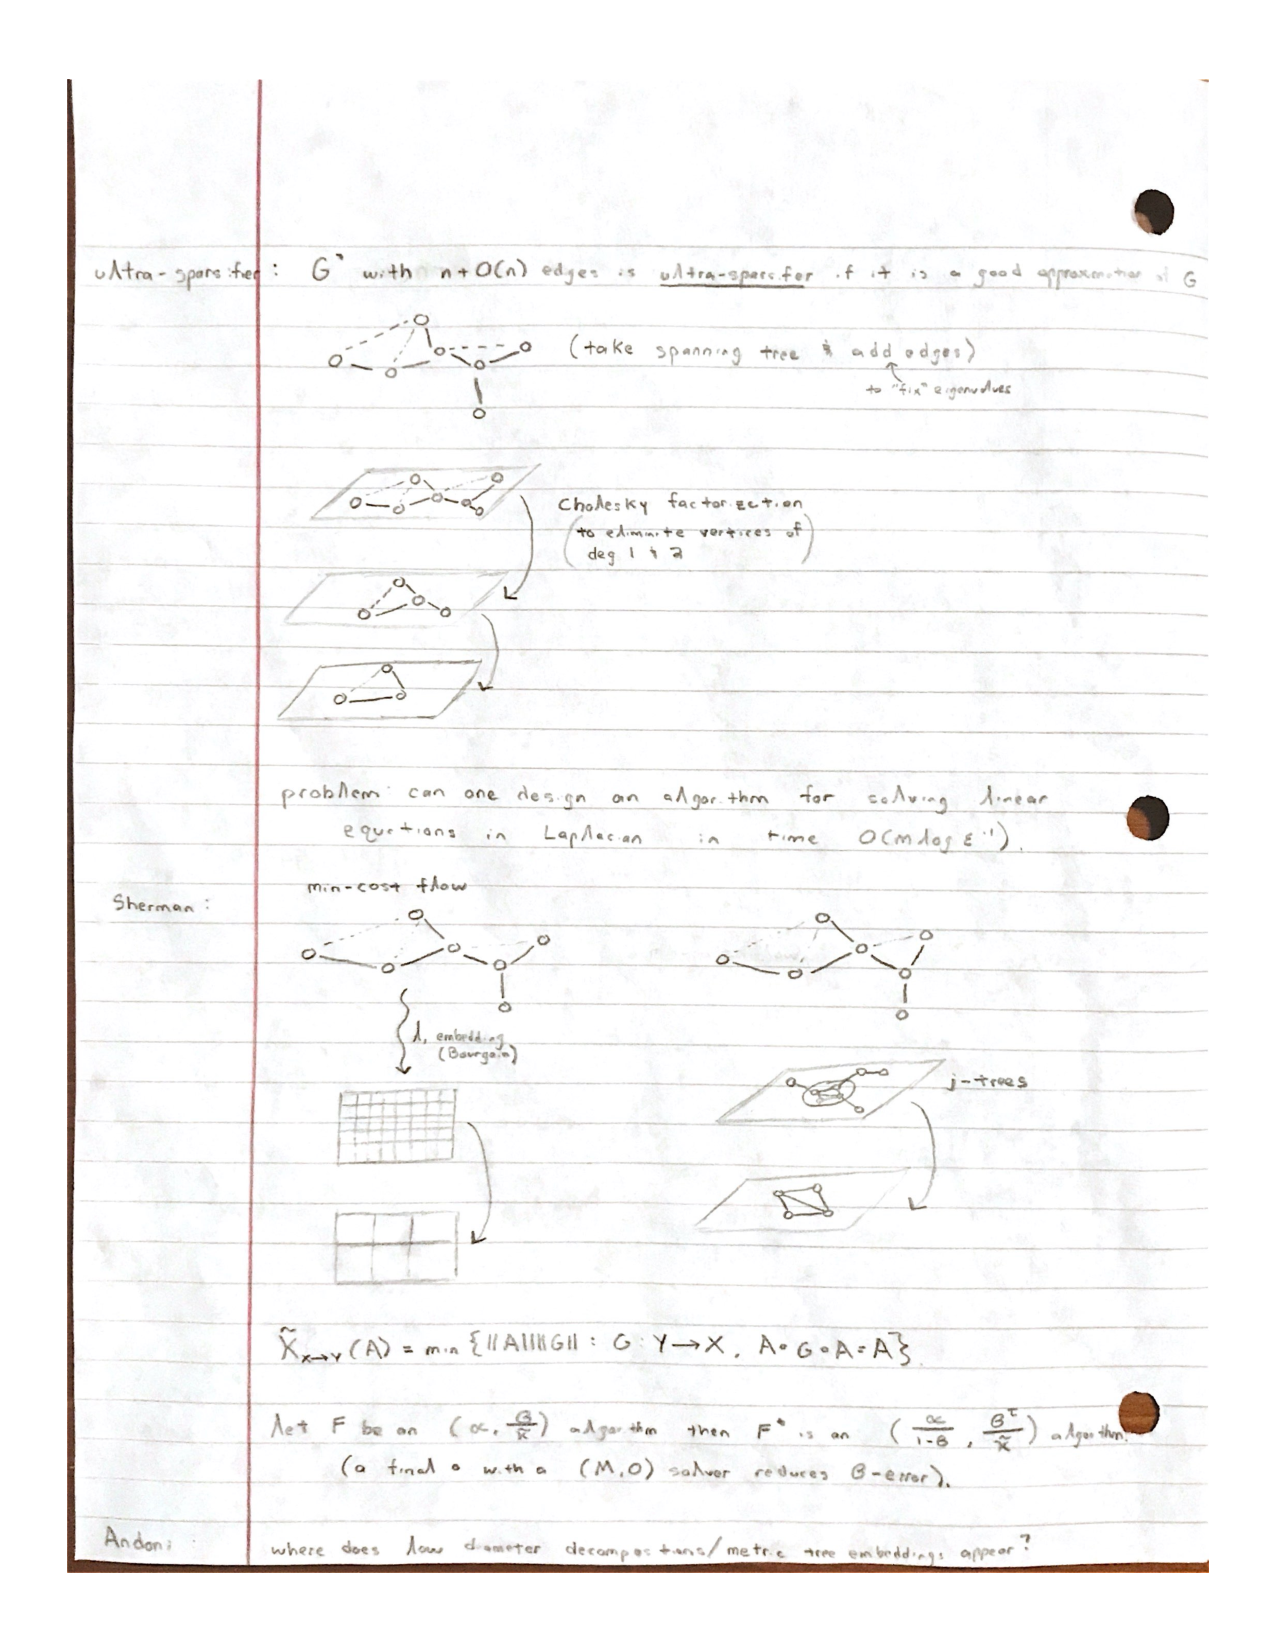
\includegraphics[width=1.0\textwidth]{../assets/drawing}
\end{figure}

\end{document}
